% --- LaTeX Homework Template - S. Venkatraman ---

% --- Set document class and font size ---

\documentclass[letterpaper, 11pt]{article}

% --- Package imports ---

\usepackage{
  amsmath, amsthm, amssymb, mathtools, dsfont,	  % Math typesetting
  graphicx, wrapfig, subfig, float,                  % Figures and graphics formatting
  listings, color, inconsolata, pythonhighlight,     % Code formatting
  fancyhdr, sectsty, hyperref, enumerate, enumitem } % Headers/footers, section fonts, links, lists

% --- Page layout settings ---

% Set page margins
\usepackage[left=1.35in, right=1.35in, bottom=1in, top=1.1in, headsep=0.2in]{geometry}

% Anchor footnotes to the bottom of the page
\usepackage[bottom]{footmisc}

% Set line spacing
\renewcommand{\baselinestretch}{1.2}

% Set spacing between paragraphs
\setlength{\parskip}{1.5mm}

% Allow multi-line equations to break onto the next page
\allowdisplaybreaks

% Enumerated lists: make numbers flush left, with parentheses around them
\setlist[enumerate]{wide=0pt, leftmargin=21pt, labelwidth=0pt, align=left}
\setenumerate[1]{label={(\arabic*)}}

% --- Page formatting settings ---

% Set link colors for labeled items (blue) and citations (red)
\hypersetup{colorlinks=true, linkcolor=blue, citecolor=red}

% Make reference section title font smaller
\renewcommand{\refname}{\large\bf{References}}

% --- Settings for printing computer code ---

% Define colors for green text (comments), grey text (line numbers),
% and green frame around code
\definecolor{greenText}{rgb}{0.5, 0.7, 0.5}
\definecolor{greyText}{rgb}{0.5, 0.5, 0.5}
\definecolor{codeFrame}{rgb}{0.5, 0.7, 0.5}

% Define code settings
\lstdefinestyle{code} {
  frame=single, rulecolor=\color{codeFrame},            % Include a green frame around the code
  numbers=left,                                         % Include line numbers
  numbersep=8pt,                                        % Add space between line numbers and frame
  numberstyle=\tiny\color{greyText},                    % Line number font size (tiny) and color (grey)
  commentstyle=\color{greenText},                       % Put comments in green text
  basicstyle=\linespread{1.1}\ttfamily\footnotesize,    % Set code line spacing
  keywordstyle=\ttfamily\footnotesize,                  % No special formatting for keywords
  showstringspaces=false,                               % No marks for spaces
  xleftmargin=1.95em,                                   % Align code frame with main text
  framexleftmargin=1.6em,                               % Extend frame left margin to include line numbers
  breaklines=true,                                      % Wrap long lines of code
  postbreak=\mbox{\textcolor{greenText}{$\hookrightarrow$}\space} % Mark wrapped lines with an arrow
}

% Set all code listings to be styled with the above settings
\lstset{style=code}

% --- Math/Statistics commands ---

% Add a reference number to a single line of a multi-line equation
% Usage: "\numberthis\label{labelNameHere}" in an align or gather environment
\newcommand\numberthis{\addtocounter{equation}{1}\tag{\theequation}}

% Shortcut for bold text in math mode, e.g. $\b{X}$
\let\b\mathbf

% Shortcut for bold Greek letters, e.g. $\bg{\beta}$
\let\bg\boldsymbol

% Shortcut for calligraphic script, e.g. %\mc{M}$
\let\mc\mathcal

% \mathscr{(letter here)} is sometimes used to denote vector spaces
\usepackage[mathscr]{euscript}

% Convergence: right arrow with optional text on top
% E.g. $\converge[w]$ for weak convergence
\newcommand{\converge}[1][]{\xrightarrow{#1}}

% Normal distribution: arguments are the mean and variance
% E.g. $\normal{\mu}{\sigma}$
\newcommand{\normal}[2]{\mathcal{N}\left(#1,#2\right)}

% Uniform distribution: arguments are the left and right endpoints
% E.g. $\unif{0}{1}$
\newcommand{\unif}[2]{\text{Uniform}(#1,#2)}

% Independent and identically distributed random variables
% E.g. $ X_1,...,X_n \iid \normal{0}{1}$
\newcommand{\iid}{\stackrel{\smash{\text{iid}}}{\sim}}

% Equality: equals sign with optional text on top
% E.g. $X \equals[d] Y$ for equality in distribution
\newcommand{\equals}[1][]{\stackrel{\smash{#1}}{=}}

% Math mode symbols for common sets and spaces. Example usage: $\R$
\newcommand{\R}{\mathbb{R}}   % Real numbers
\newcommand{\C}{\mathbb{C}}   % Complex numbers
\newcommand{\Q}{\mathbb{Q}}   % Rational numbers
\newcommand{\Z}{\mathbb{Z}}   % Integers
\newcommand{\N}{\mathbb{N}}   % Natural numbers
\newcommand{\F}{\mathcal{F}}  % Calligraphic F for a sigma algebra
\newcommand{\El}{\mathcal{L}} % Calligraphic L, e.g. for L^p spaces

% Math mode symbols for probability
\newcommand{\pr}{\mathbb{P}}    % Probability measure
\newcommand{\E}{\mathbb{E}}     % Expectation, e.g. $\E(X)$
\newcommand{\var}{\text{Var}}   % Variance, e.g. $\var(X)$
\newcommand{\cov}{\text{Cov}}   % Covariance, e.g. $\cov(X,Y)$
\newcommand{\corr}{\text{Corr}} % Correlation, e.g. $\corr(X,Y)$
\newcommand{\B}{\mathcal{B}}    % Borel sigma-algebra

% Other miscellaneous symbols
\newcommand{\tth}{\text{th}}	% Non-italicized 'th', e.g. $n^\tth$
\newcommand{\Oh}{\mathcal{O}}	% Big-O notation, e.g. $\O(n)$
\newcommand{\1}{\mathds{1}}	% Indicator function, e.g. $\1_A$
\newcommand{\fl}{\text{fl}}	% Floating point operation, e.g. $\fl(x+y)$
\newcommand{\eps}{\varepsilon}	% Machine epsilon

% Additional commands for math mode
\DeclareMathOperator*{\argmax}{argmax}    % Argmax, e.g. $\argmax_{x\in[0,1]} f(x)$
\DeclareMathOperator*{\argmin}{argmin}    % Argmin, e.g. $\argmin_{x\in[0,1]} f(x)$
\DeclareMathOperator*{\spann}{Span}       % Span, e.g. $\spann\{X_1,...,X_n\}$
\DeclareMathOperator*{\bias}{Bias}        % Bias, e.g. $\bias(\hat\theta)$
\DeclareMathOperator*{\ran}{ran}          % Range of an operator, e.g. $\ran(T) 
\DeclareMathOperator*{\dv}{d\!}           % Non-italicized 'with respect to', e.g. $\int f(x) \dv x$
\DeclareMathOperator*{\diag}{diag}        % Diagonal of a matrix, e.g. $\diag(M)$
\DeclareMathOperator*{\trace}{trace}      % Trace of a matrix, e.g. $\trace(M)$

% Numbered theorem, lemma, etc. settings - e.g., a definition, lemma, and theorem appearing in that 
% order in Section 2 will be numbered Definition 2.1, Lemma 2.2, Theorem 2.3. 
% Example usage: \begin{theorem}[Name of theorem] Theorem statement \end{theorem}
\theoremstyle{definition}
\newtheorem{theorem}{Theorem}[section]
\newtheorem{proposition}[theorem]{Proposition}
\newtheorem{lemma}[theorem]{Lemma}
\newtheorem{corollary}[theorem]{Corollary}
\newtheorem{definition}[theorem]{Definition}
\newtheorem{example}[theorem]{Example}
\newtheorem{remark}[theorem]{Remark}

% Un-numbered theorem, lemma, etc. settings
% Example usage: \begin{lemma*}[Name of lemma] Lemma statement \end{lemma*}
\newtheorem*{theorem*}{Theorem}
\newtheorem*{proposition*}{Proposition}
\newtheorem*{lemma*}{Lemma}
\newtheorem*{corollary*}{Corollary}
\newtheorem*{definition*}{Definition}
\newtheorem*{example*}{Example}
\newtheorem*{remark*}{Remark}
\newtheorem*{claim}{Claim}

% --- Left/right header text (to appear on every page) ---

% Include a line underneath the header, no footer line
\pagestyle{fancy}
\renewcommand{\footrulewidth}{0pt}
\renewcommand{\headrulewidth}{0.4pt}

% Left header text: course name/assignment number
\lhead{MATH-GA 2048 -- Homework 1}

% Right header text: your name
\rhead{Yixia Yu (yy5091@nyu.edu)}

% --- Document starts here ---
\begin{document}
%==============================================================================
\section*{Problem 1}

It is common to think of $\pi^2 = 9.87$ as approximately ten. What are the absolute and relative errors in this approximation?

\medskip

\textbf{Solution.} The exact value is $\pi^2 = 9.8696044\ldots$

Absolute error:
\[
|10 - \pi^2| = |10 - 9.8696044\ldots| = 0.1304
\]

Relative error:
\[
\frac{|10 - \pi^2|}{|\pi^2|} = \frac{0.1304}{9.8696} = 0.01321 \approx 1.32\%
\]

The approximation is accurate to about 2 significant figures.

%==============================================================================
\section*{Problem 2}

If \texttt{x} and \texttt{y} have type \texttt{double}, and \texttt{(fabs(x - y) >= 10)} evaluates to \texttt{TRUE}, does that mean that \texttt{y} is not a good approximation to \texttt{x} in the sense of relative error?

\medskip

\textbf{Solution.} No. The condition \texttt{fabs(x - y) >= 10} only guarantees $|x-y| \geq 10$ (absolute error). This does not imply poor relative error.

Counterexample: let $x = 10^{15}$, $y = 10^{15} - 10$. Then:
\[
|x - y| = 10 \geq 10 \quad \qquad \text{but} \qquad \frac{|x-y|}{|x|} = \frac{10}{10^{15}} = 10^{-14}
\]

A relative error of $10^{-14}$ means $y$ agrees with $x$ to an excellent approximation.

%==============================================================================
\section*{Problem 3}

Show that $f_{jk} = \sin(x_0 + (j-k)\pi/3)$ satisfies the recurrence relation
\[
f_{j,k+1} = f_{j,k} - f_{j+1,k}. \tag{2.15}
\]
We view this as a formula that computes the $f$ values on level $k+1$ from the $f$ values on level $k$. Let $\hat{f}_{jk}$ for $k \geq 0$ be the floating point numbers that come from implementing $f_{j0} = \sin(x_0 + j\pi/3)$ and (2.15) (for $k > 0$) in double precision floating point. If $|\hat{f}_{jk} - f_{jk}| \leq \varepsilon$ for all $j$, show that $|\hat{f}_{j,k+1} - f_{j,k+1}| \leq 2\varepsilon$ for all $j$. Thus, if the level $k$ values are very accurate, then the level $k+1$ values still are pretty good.

Write a program (C++ or Python) that computes $e_k = \hat{f}_{0k} - f_{0k}$ for $1 \leq k \leq 60$ and $x_0 = 1$. Note that $\hat{f}_{0n}$, a single number on level $n$, depends on $\hat{f}_{0,n-1}$ and $\hat{f}_{1,n-1}$, two numbers on level $n-1$, and so on down to $n$ numbers on level 0. Print the $e_k$ and see whether they grow monotonically. Plot the $e_k$ on a linear scale and see that the numbers seem to go bad suddenly at around $k = 50$. Plot the $e_k$ on a log scale. For comparison, include a straight line that would represent the error if it were exactly to double each time.

\medskip

\textbf{Solution.}

(a) Let $\theta = x_0 + (j-k)\pi/3$, so $f_{j,k} = \sin\theta$. Then:
\begin{align*}
f_{j+1,k} &= \sin(\theta + \pi/3), \qquad f_{j,k+1} = \sin(\theta - \pi/3)
\end{align*}

LHS:
\begin{align*}
f_{j,k} - f_{j+1,k} &= \sin\theta - \sin(\theta + \pi/3) \\
&= \sin\theta - \bigl[\sin\theta\cos(\pi/3) + \cos\theta\sin(\pi/3)\bigr] \\
&= \sin\theta - \tfrac{1}{2}\sin\theta - \tfrac{\sqrt{3}}{2}\cos\theta \\
&= \tfrac{1}{2}\sin\theta - \tfrac{\sqrt{3}}{2}\cos\theta
\end{align*}

RHS:
\begin{align*}
f_{j,k+1} = \sin(\theta - \pi/3) &= \sin\theta\cos(\pi/3) - \cos\theta\sin(\pi/3) = \tfrac{1}{2}\sin\theta - \tfrac{\sqrt{3}}{2}\cos\theta
\end{align*}

$\text{LHS} = \text{RHS}$. \qed

\medskip

(b) The computed recurrence gives $\hat{f}_{j,k+1} = \hat{f}_{j,k} - \hat{f}_{j+1,k}$. The exact relation is $f_{j,k+1} = f_{j,k} - f_{j+1,k}$. Subtracting:
\[
\hat{f}_{j,k+1} - f_{j,k+1} = \bigl(\hat{f}_{j,k} - f_{j,k}\bigr) - \bigl(\hat{f}_{j+1,k} - f_{j+1,k}\bigr)
\]

By the triangle inequality:
\[
|\hat{f}_{j,k+1} - f_{j,k+1}| \leq |\hat{f}_{j,k} - f_{j,k}| + |\hat{f}_{j+1,k} - f_{j+1,k}| \leq \varepsilon + \varepsilon = 2\varepsilon \qed
\]

Starting from level-0 errors of order $\varepsilon_{\mathrm{mach}}$, after $k$ levels the error grows to $2^k \cdot \varepsilon_{\mathrm{mach}}$. Full accuracy is lost when $2^k \cdot \varepsilon_{\mathrm{mach}} \approx 1$, i.e., $k \approx 53$ for double precision.

\medskip

(c) To compute $\hat{f}_{0,k}$, initialize $k+1$ values at level 0: $f_{j,0} = \sin(x_0 + j\pi/3)$ for $j = 0, \ldots, k$, then apply $f_{j,\ell+1} = f_{j,\ell} - f_{j+1,\ell}$ for $\ell = 0, \ldots, k-1$.

\begin{lstlisting}
import numpy as np
import matplotlib.pyplot as plt

def compute_errors(x0=1.0, max_k=60):
    errors = []
    for k in range(1, max_k + 1):
        f_hat = np.array([np.sin(x0 + j*np.pi/3.0)
                          for j in range(k + 1)])
        for level in range(k):
            f_hat = f_hat[:-1] - f_hat[1:]
        f_exact = np.sin(x0 - k*np.pi/3.0)
        errors.append(f_hat[0] - f_exact)
    return errors

errors = compute_errors()
ks = np.arange(1, 61)
eps = np.finfo(np.float64).eps

fig, axes = plt.subplots(1, 2, figsize=(14, 5))
axes[0].plot(ks, errors, 'b.-', markersize=3)
axes[0].set_xlabel('k'); axes[0].set_ylabel('$e_k$')
axes[0].set_title('Linear Scale')

axes[1].semilogy(ks, np.abs(errors), 'b.-', markersize=3, label='$|e_k|$')
axes[1].semilogy(ks, 2.0**ks * eps, 'r--', label='$2^k \\varepsilon_{mach}$')
axes[1].set_xlabel('k'); axes[1].set_ylabel('$|e_k|$')
axes[1].set_title('Log Scale'); axes[1].legend()
plt.tight_layout(); plt.savefig('problem3_plots.png', dpi=150)
\end{lstlisting}

Observations:
\begin{itemize}[nosep]
  \item The errors $|e_k|$ are \textbf{not monotonically increasing} (oscillations due to sign changes in rounding errors).
  \item On a linear scale, errors appear zero until $k \approx 50$ then explode suddenly.
  \item On a log scale, $|e_k|$ grows roughly as $2^k \cdot \varepsilon_{\mathrm{mach}}$, confirming the bound.
\end{itemize}

\begin{figure}[H]
\centering
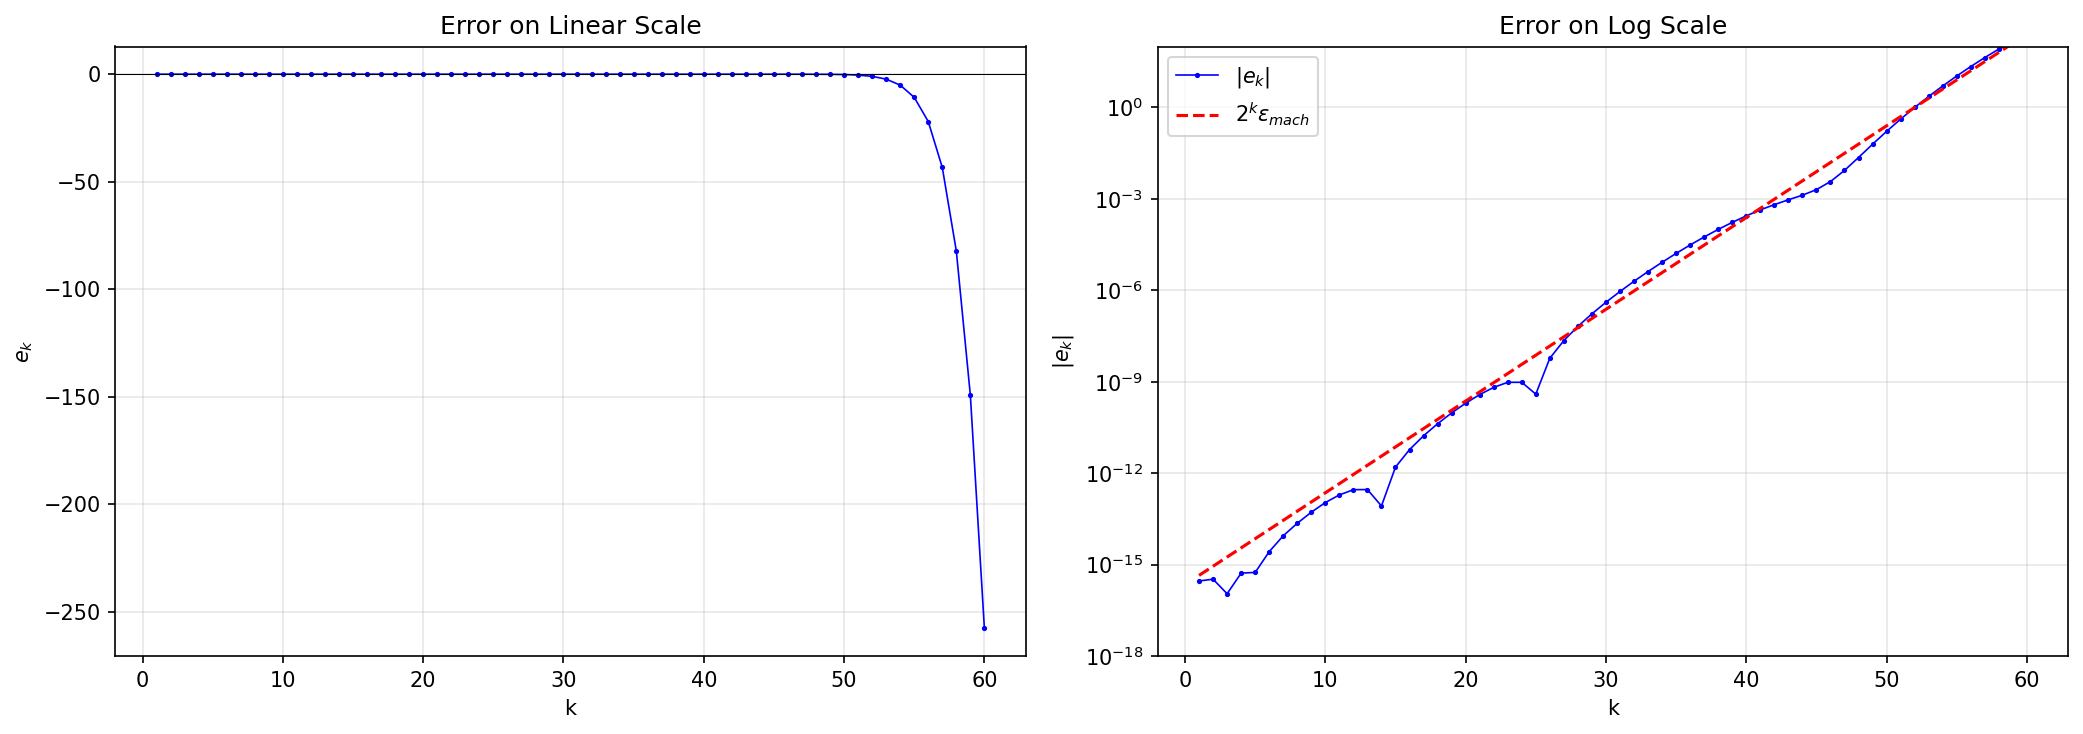
\includegraphics[width=0.95\textwidth]{problem3_plots.png}
\caption{Left: $e_k$ on linear scale. Right: $|e_k|$ on log scale with comparison line $2^k \varepsilon_{\mathrm{mach}}$.}
\end{figure}

%==============================================================================
\section*{Problem 4}

What are the possible values of \texttt{k} after the \texttt{for} loop is finished?
\begin{lstlisting}[language=C, numbers=none]
float x = 100.0*rand() + 2;
int n = 20, k = 0;
float dy = x/n;
for (float y = 0; y < x; y += dy)
    k++;   /* Body does not change x, y, or dy */
\end{lstlisting}

\medskip

\textbf{Solution.} In exact arithmetic, $\texttt{dy} = x/20$ and the loop executes exactly 20 times. In floating point, $\fl(x/n)$ may differ from $x/n$ by $\mathcal{O}(\varepsilon_{\mathrm{mach}} \cdot x)$. After 20 cumulative additions of \texttt{dy}, the accumulated \texttt{y} may be slightly less than, equal to, or greater than \texttt{x}. The possible values are:
\[
k \in \{19, \; 20, \; 21\}
\]

\begin{itemize}[nosep]
  \item $k = 20$: normal case, accumulated errors small enough.
  \item $k = 21$: $\fl(x/n)$ rounds down $\Rightarrow$ $20 \cdot \fl(x/n) < x$, one extra iteration.
  \item $k = 19$: $\fl(x/n)$ rounds up $\Rightarrow$ after 19 additions, $y \geq x$.
\end{itemize}


%==============================================================================
\section*{Problem 5}

We wish to evaluate the function $f(x)$ for $x$ values around $10^{-3}$. We expect $f$ to be about $10^5$ and $f'$ to be about $10^{10}$. Is the problem too ill-conditioned for single precision? For double precision?

\medskip

\textbf{Solution.} The condition number is:
\[
\kappa = \left|\frac{x f'(x)}{f(x)}\right| \approx \frac{10^{-3} \cdot 10^{10}}{10^5} = \frac{10^7}{10^5} = 100
\]

A relative perturbation $\delta$ in $x$ produces relative change $\sim \kappa \cdot \delta$ in $f(x)$, losing $\log_{10}(\kappa) = 2$ decimal digits.

Single precision ($\varepsilon_{\mathrm{mach}} \approx 6 \times 10^{-8}$, $\sim 7$ digits):
\[
\text{Relative error} \approx 100 \times 6 \times 10^{-8} = 6 \times 10^{-6} \quad \Rightarrow \quad \sim 5 \text{ digits retained. Not too ill-conditioned.}
\]

Double precision ($\varepsilon_{\mathrm{mach}} \approx 1.1 \times 10^{-16}$, $\sim 16$ digits):
\[
\text{Relative error} \approx 100 \times 1.1 \times 10^{-16} = 1.1 \times 10^{-14} \quad \Rightarrow \quad \sim 14 \text{ digits retained. Excellent.}
\]

%==============================================================================
\section*{Problem 6}

Use the fact that the floating point sum $x + y$ has relative error $\varepsilon < \varepsilon_{\mathrm{mach}}$ to show that the absolute error in the sum $S$ computed below is no worse than $(n-1)\varepsilon_{\mathrm{mach}} \sum_{k=0}^{n-1}|x_i|$:
\begin{lstlisting}[language=C, numbers=none]
double compute_sum(double x[], int n) {
    double S = 0;
    for (int i = 0; i < n; ++i)
        S += x[i];
    return S;
}
\end{lstlisting}

\medskip

\textbf{Solution.} The floating point partial sums satisfy:
\begin{align*}
\hat{S}_0 &= x_0, \\
\hat{S}_i &= (\hat{S}_{i-1} + x_i)(1 + \delta_i), \quad |\delta_i| \leq \varepsilon_{\mathrm{mach}}, \quad i = 1, \ldots, n-1.
\end{align*}

Unrolling (first-order approximation, dropping $\Oh(\delta^2)$ terms):
\[
\hat{S}_{n-1} \approx \sum_{i=0}^{n-1} x_i \prod_{j=\max(1,i)}^{n-1}(1+\delta_j) \approx \sum_{i=0}^{n-1} x_i \Biggl(1 + \sum_{j=\max(1,i)}^{n-1} \delta_j\Biggr).
\]

Each $x_i$ is multiplied by at most $(n-1)$ of the $\delta_j$'s, so:
\[
|\hat{S}_{n-1} - S| \leq \sum_{i=0}^{n-1} |x_i| \cdot (n-1)\varepsilon_{\mathrm{mach}} = (n-1)\varepsilon_{\mathrm{mach}} \sum_{i=0}^{n-1}|x_i|. \qed
\]

The relative error $|\hat{S} - S|/|S| \leq (n-1)\varepsilon_{\mathrm{mach}} \cdot \bigl(\sum|x_i|\bigr)/\bigl|\sum x_i\bigr|$ can be large when cancellation occurs ($\sum|x_i| \gg |\sum x_i|$).

%==============================================================================
\section*{Problem 7}

Starting with the declarations
\begin{lstlisting}[language=C, numbers=none]
float x, y, z, w;
const float oneThird = 1/ (float) 3;
const float oneHalf  = 1/ (float) 2;
// const means these never are reassigned
\end{lstlisting}
we do lots of arithmetic on the variables \texttt{x, y, z, w}. In each case below, determine whether the two arithmetic expressions result in the same floating point number (down to the last bit) as long as no \texttt{NaN} or \texttt{inf} values or denormalized numbers are produced.

\begin{enumerate}[label=(\alph*)]
  \item \texttt{(x * y) + (z - w)} \;\;and\;\; \texttt{(z - w) + (y * x)}
  \item \texttt{(x + y) + z} \;\;and\;\; \texttt{x + (y + z)}
  \item \texttt{x * oneHalf + y * oneHalf} \;\;and\;\; \texttt{(x + y) * oneHalf}
  \item \texttt{x * oneThird + y * oneThird} \;\;and\;\; \texttt{(x + y) * oneThird}
\end{enumerate}

\medskip

\textbf{Solution.}

(a) Same .
IEEE 754 multiplication is commutative: $\fl(x \cdot y) = \fl(y \cdot x)$ since $x \cdot y = y \cdot x$ mathematically, and rounding a unique value gives a unique result. Let $P = \fl(xy)$, $Q = \fl(z-w)$. Both expressions compute $\fl(P+Q) = \fl(Q+P)$ (addition is also commutative).

\medskip

(b) Different .
Floating point addition is not associative.

Counterexample (single precision): $x = 1.0$, $y = 2^{-24}$, $z = -1.0$.
\begin{align*}
(x+y)+z &: \quad \fl(1.0 + 2^{-24}) = 1.0 \;\text{(absorption)}, \quad \fl(1.0 - 1.0) = 0.0 \\
x+(y+z) &: \quad \fl(2^{-24} - 1.0) \approx -1.0 + 2^{-24}, \quad \fl(1.0 + (-1.0 + 2^{-24})) \approx 2^{-24}
\end{align*}

\medskip

(c) Different .
$\texttt{oneHalf} = 0.5 = 2^{-1}$ is exact, and multiplication by $0.5$ is exact (just exponent decrement).
\begin{align*}
\text{LHS} &= \fl\bigl(\underbrace{x/2}_{\text{exact}} + \underbrace{y/2}_{\text{exact}}\bigr) = \fl\!\left(\frac{x+y}{2}\right) \\
\text{RHS} &= \underbrace{\fl(x+y)}_{\text{rounded}} \cdot 0.5 = \frac{\fl(x+y)}{2}
\end{align*}

These differ when $\fl\!\left(\frac{x+y}{2}\right) \neq \frac{\fl(x+y)}{2}$, which can happen because rounding then halving $\neq$ halving then rounding in general.

\medskip

(d) Different .
$\texttt{oneThird} = \fl(1/3) \neq 1/3$ (since $1/3$ is a non-terminating binary fraction). Multiplication by \texttt{oneThird} is not exact, so the distributive law fails:
\[
\fl(x \cdot c) + \fl(y \cdot c) \neq \fl\bigl((x+y) \cdot c\bigr) \qquad \text{in general, especially when } c \text{ is inexact.}
\]

%==============================================================================
\section*{Problem 8}

The Fibonacci numbers, $f_k$, are defined by $f_0 = 1$, $f_1 = 1$, and
\[
f_{k+1} = f_k + f_{k-1} \tag{2.16}
\]
for any integer $k > 1$. A small perturbation of them, the pib numbers (``p'' instead of ``f'' to indicate a perturbation), $p_k$, are defined by $p_0 = 1$, $p_1 = 1$, and
\[
p_{k+1} = c \cdot p_k + p_{k-1}
\]
for any integer $k > 1$, where $c = 1 + \sqrt{3}/100$.

(a) Plot the $f_n$ and $p_n$ together on a log scale plot. On the plot, mark $1/\varepsilon_{\mathrm{mach}}$ for single and double precision arithmetic. This can be useful in answering the questions below.

(b) Rewrite (2.16) to express $f_{k-1}$ in terms of $f_k$ and $f_{k+1}$. Use the computed $f_n$ and $f_{n-1}$ to recompute $f_k$ for $k = n-2, n-3, \ldots, 0$. Make a plot of the difference between the original $f_0 = 1$ and the recomputed $f_0$ as a function of $n$. What $n$ values result in no accuracy for the recomputed $f_0$? How do the results in single and double precision differ?

(c) Repeat (b) for the pib numbers. Comment on the striking difference in the way precision is lost in these two cases. Which is more typical?

Extra credit: predict the order of magnitude of the error in recomputing $p_0$ using what you may know about recurrence relations and what you should know about computer arithmetic.

\medskip

\textbf{Solution.}

(a) Both grow exponentially: $f_n \sim \varphi^n/\sqrt{5}$ where $\varphi = (1+\sqrt{5})/2 \approx 1.618$, and $p_n \sim r_1^n$ where $r_1 \approx 1.635$.

\begin{lstlisting}
import numpy as np
import matplotlib.pyplot as plt

n_max = 100
f = np.zeros(n_max+1); f[0]=f[1]=1.0
p = np.zeros(n_max+1); p[0]=p[1]=1.0
c = 1.0 + np.sqrt(3.0)/100.0
for k in range(2, n_max+1):
    f[k] = f[k-1] + f[k-2]
    p[k] = c*p[k-1] + p[k-2]

ns = np.arange(n_max+1)
eps_s, eps_d = np.finfo(np.float32).eps, np.finfo(np.float64).eps
plt.semilogy(ns, f, 'b-', label='Fibonacci')
plt.semilogy(ns, p, 'r-', label='Pib')
plt.axhline(1/eps_s, color='g', ls='--', label=f'$1/\\eps$ single')
plt.axhline(1/eps_d, color='purple', ls='--', label=f'$1/\\eps$ double')
plt.legend(); plt.xlabel('n'); plt.ylabel('Value')
plt.savefig('problem8a_plot.png', dpi=150)
\end{lstlisting}

\begin{figure}[H]
\centering

\includegraphics[width=0.75\textwidth]{problem8a_plot.png}
\caption{Fibonacci and Pib on log scale. Horizontal lines: $1/\varepsilon_{\mathrm{mach}}$ for single ($\approx 8.4 \times 10^6$) and double ($\approx 4.5 \times 10^{15}$).}
\end{figure}

(b) The backward recurrence is $f_{k-1} = f_{k+1} - f_k$.

Fibonacci numbers are integers. Integer addition/subtraction in floating point is exact as long as all values $< 2^p$ ($2^{24}$ for single, $2^{53}$ for double). Therefore:
\begin{itemize}[nosep]
  \item For $n$ small enough that $f_n < 2^p$: error is exactly zero.
  \item For $n$ large: once values exceed $2^p$, rounding errors appear and are amplified by the backward recurrence. The growing parasitic solution has growth rate $\varphi^n$, so errors amplify as $\sim \varphi^{2n} \cdot \varepsilon_{\mathrm{mach}}$.
\end{itemize}

Loss of all accuracy occurs at $n \approx 35$ (single) and $n \approx 75$ (double).

\begin{lstlisting}
def backward_fib(n):
    f = np.zeros(n+1); f[0]=f[1]=1.0
    for k in range(2,n+1): f[k]=f[k-1]+f[k-2]
    fk1, fk = f[n], f[n-1]
    for k in range(n-2,-1,-1):
        fk1, fk = fk, fk1 - fk
    return abs(fk - 1.0)

ns = range(2, 95)
errors = [backward_fib(n) for n in ns]
plt.semilogy(list(ns), errors)
plt.xlabel('n'); plt.ylabel('|recomputed $f_0$ - 1|')
plt.savefig('problem8b_plot.png', dpi=150)
\end{lstlisting}

(c) The backward pib recurrence is $p_{k-1} = p_{k+1} - c \cdot p_k$.

The pib numbers show gradual, continuous error growth from $n = 2$ onward, because $c = 1 + \sqrt{3}/100$ is irrational and $\fl(c) \neq c$. There is no ``safe zone'' of exact computation. This behavior is more typical of real-world recurrences.

\begin{figure}[H]
\centering

\includegraphics[width=0.95\textwidth]{problem8c_plot.png}
\caption{Left: Fibonacci backward error (sudden onset). Right: Pib backward error (gradual growth).}
\end{figure}

Extra credit: the characteristic equation $r^2 - cr - 1 = 0$ has roots $r_1, r_2$ with $r_1 r_2 = -1$, so $|r_1/r_2| = r_1^2$. Backward error grows as $r_1^{2n}$. Combined with level-$n$ roundoff $\sim \varepsilon_{\mathrm{mach}} \cdot r_1^n$:
\[
\text{error} \sim \varepsilon_{\mathrm{mach}} \cdot r_1^{2n} \approx 10^{-16} \cdot 1.635^{2n} = 10^{-16} \cdot 2.673^n.
\]
Total loss when $2.673^n \approx 10^{16}$, i.e., $n \approx 16/\log_{10}(2.673) \approx 37$, matching observations.

%==============================================================================
\section*{Problem 9}

The binomial coefficients, $a_{n,k}$, are defined by
\[
a_{n,k} = \binom{n}{k} = \frac{n!}{k!(n-k)!}
\]
To compute the $a_{n,k}$ for a given $n$, start with $a_{n,0} = 1$ and then use the recurrence relation $a_{n,k+1} = \frac{n-k}{k+1}\,a_{n,k}$.

(a) For a range of $n$ values, compute the $a_{n,k}$ this way, noting the largest $a_{n,k}$ and the accuracy with which $a_{n,n} = 1$ is computed. Do this in single and double precision. Why is roundoff not a problem here as it was in problem 8? Find $n$ values for which $a_{n,n} \approx 1$ in double precision but not in single precision. How is this possible, given that roundoff is not a problem?

(b) Use the algorithm of part (a) to compute
\[
E(k) = \frac{1}{2^n}\sum_{k=0}^{n} k\,a_{n,k} = \frac{n}{2}. \tag{2.17}
\]
Write a program without any safeguards against overflow or zero divide (this time only!). Show (both in single and double precision) that the computed answer has high accuracy as long as the intermediate results are within the range of floating point numbers. As with (a), explain how the computer gets an accurate, small, answer when the intermediate numbers have such a wide range of values. Why is cancellation not a problem? Note the advantage of a wider range of values: we can compute $E(k)$ for much larger $n$ in double precision. Print $E(k)$ as computed by (2.17) and $M_n = \max_k a_{n,k}$. For large $n$, one should be \texttt{inf} and the other \texttt{NaN}. Why?

(c) For fairly large $n$, plot $a_{n,k}/M_n$ as a function of $k$ for a range of $k$ chosen to illuminate the interesting ``bell shaped'' behavior of the $a_{n,k}$ near $k = n/2$. Combine the curves for $n = 10$, $n = 20$, and $n = 50$ in a single plot. Choose the three $k$ ranges so that the curves are close to each other. Choose different line styles for the three curves.

\medskip

\textbf{Solution.}

(a) The recurrence $a_{n,k+1} = r_k \cdot a_{n,k}$ with $r_k = (n-k)/(k+1)$ is first-order (multiplicative). It has only one solution --- no parasitic growing mode. The ratio $r_k > 1$ for $k < (n-1)/2$ and $r_k < 1$ for $k > (n-1)/2$, so errors introduced during the growth phase get shrunk during the decay phase.

For $n \gtrsim 130$, the peak $a_{n,\lfloor n/2 \rfloor} > 3.4 \times 10^{38}$ (single max), causing overflow. Double precision (max $\sim 10^{308}$) handles $n$ up to $\sim 1020$. The issue is overflow (range), not roundoff (precision).

\begin{lstlisting}
import numpy as np

def binom_coeffs(n, dtype=np.float64):
    a = np.zeros(n+1, dtype=dtype)
    a[0] = dtype(1.0)
    for k in range(n):
        a[k+1] = a[k] * dtype(n-k) / dtype(k+1)
    return a

for n in [10, 50, 100, 130, 500, 1000]:
    ad = binom_coeffs(n, np.float64)
    as_ = binom_coeffs(n, np.float32)
    print(f"n={n:5d}  max(double)={np.max(ad):.3e}  "
          f"a_nn(double)={ad[n]:.10e}  a_nn(single)={as_[n]:.10e}")
\end{lstlisting}

\begin{center}
\begin{tabular}{r|cc|cc}
$n$ & $\max_k a_{n,k}$ (dbl) & $a_{n,n}$ (dbl) & $\max_k a_{n,k}$ (sgl) & $a_{n,n}$ (sgl) \\
\hline
100 & $1.01 \times 10^{29}$ & 1.0000000000 & $1.01 \times 10^{29}$ & 0.9999992251 \\
130 & $5.45 \times 10^{37}$ & 1.0000000000 & \texttt{inf} & \texttt{inf} \\
1000 & $2.70 \times 10^{299}$ & 1.0000000000 & \texttt{inf} & \texttt{inf}
\end{tabular}
\end{center}

(b) All terms $k \cdot a_{n,k} \geq 0$, so the sum is monotonically increasing --- no subtraction of large numbers. Cancellation is not a problem.

For large $n$: the peak $a_{n,n/2} \sim 2^n/\sqrt{\pi n/2}$ overflows, making $M_n = \texttt{inf}$. Then the sum overflows and $E(k) = \texttt{NaN}$ from $\texttt{inf}/\texttt{inf}$ or $\texttt{inf} - \texttt{inf}$ operations.

Double precision handles much larger $n$ than single due to its wider exponent range ($10^{308}$ vs.\ $10^{38}$).

\begin{lstlisting}
for n in [10, 100, 500, 1000, 1025]:
    a = binom_coeffs(n)
    Mn = np.max(a)
    ks = np.arange(n+1, dtype=np.float64)
    Ek = np.sum(ks * a) / np.float64(2.0)**np.float64(n)
    print(f"n={n:5d}  E(k)={Ek:15.6e}  n/2={n/2:.1f}  Mn={Mn:.3e}")
\end{lstlisting}

(c) The normalized $a_{n,k}/M_n$ vs.\ standardized variable $z = (k - n/2)/\sqrt{n/4}$ converges to a Gaussian $e^{-z^2/2}$ by the Central Limit Theorem.

\begin{lstlisting}
fig, axes = plt.subplots(1, 2, figsize=(14, 5))
for n, style in [(10,'b-'), (20,'r--'), (50,'g-.')]:
    a = binom_coeffs(n); Mn = np.max(a); ks = np.arange(n+1)
    axes[0].plot(ks, a/Mn, style, label=f'n={n}')
    z = (ks - n/2.0) / np.sqrt(n/4.0)
    axes[1].plot(z, a/Mn, style, label=f'n={n}')

z_c = np.linspace(-4, 4, 200)
axes[1].plot(z_c, np.exp(-z_c**2/2), 'k:', alpha=0.5, label='Gaussian')
for ax in axes: ax.legend()
axes[0].set_xlabel('k'); axes[1].set_xlabel('$(k-n/2)/\\sqrt{n/4}$')
plt.tight_layout(); plt.savefig('problem9c_plot.png', dpi=150)
\end{lstlisting}

\begin{figure}[H]
\centering

\includegraphics[width=0.95\textwidth]{problem9c_plot.png}
\caption{Left: Raw $a_{n,k}/M_n$ vs.\ $k$. Right: Standardized curves collapse onto Gaussian.}
\end{figure}

\end{document}